
\chapter{État de l'art des technologies}

\section{Présentation du contexte}

Dans le domaine de la détection de drones, après recherche littéraires et numérique, nous en avons conclu qu'il existait plusieurs types de détection: par acoustique, par méthodes optiques et par radiogoniométrie.
Ces méthodes possèdent chacunes leurs avantages et leurs inconvéniants que nous allons spécifier ci-dessous.


\section{Acoustique}

Plusieurs entreprises proposent des outils de détection des drones. Ces derniers se présentent sous forme de boîtiers reliés à des micros, positionnés en hauteur: c'est par le son de leurs hélices que les drones sont repérés, dans un rayon d'une centaine de mètres. Une alerte est alors envoyée sur un ordinateur ou par un SMS. Avantage: le système ne s'occupe pas des ondes, et peut détecter les drones autopilotés (voir plus bas). Problème: le bruit de fond doit être inférieur à un certain seuil, ce qui le rend difficilement utilisable en milieu urbain. De plus, pour des raisons d'échos, la multiplication de récepteurs est nécessaire afin de pouvoir filtrer le signal. Enfin, il est nécessaire de disposer préalablement d'une base de données des signatures acoustiques des différents drones qui peuvent émettre sur un domaine de fréquences acoustiques larges.

Cependant, ce système présente des failles. En effet, il est assez simple pour un drone de parer ce système de détection. Par la simple émission d'une onde sonore couvrant sa propre signature acoustique, un drone passerait totalement inaperçu.

Certains systèmes utilisent aussi une analyse fréquentielle poussée du signal afin de détecter les moteurs en fonction de leurs fréquences de fonctionnement.

Au-delà de cet aspect, il présente un avantage et des plus importants, son coût. En effet, un tel système est très économique à produire. Actuellement diverses solutions actives comme passives sont déjà présentes sur le marché. Ces solutions sont orientées vers une utilisation domestique et non professionnelle pour les raisons évoquées précédemment. Leur prix se situe aux alentours de 100 dollars pour un modèle classique, mais la multiplication des solutions tant à réduire le prix d'un tel système. 

\section{Optique}

Une caméra normale a besoin de lumière pour produire une image, une caméra thermique (ou infrarouge) peut capter de très faibles différences de température et les convertir en une excellente image thermique sur laquelle les plus petits détails sont visibles. Contrairement à d'autres technologies, comme l'amplification de lumière qui nécessite une petite quantité de lumière pour produire une image, l'imagerie thermique permet de voir dans l'obscurité totale. Elle ne nécessite aucune source de lumière.

Depuis qu'il est possible de produire une image lisible dans l'obscurité totale, la technologie de l'imagerie thermique permet de voir et de cibler les forces ennemies dans la nuit la plus noire. Les caméras thermiques voient à travers la brume, la pluie et la neige. Elles voient aussi à travers la fumée, ce qui était particulièrement intéressant pour l'armée.\cite{optique}

En mode passif, \emph{des caméras thermiques d'observation savent repérer un drone de 50 cm d'envergure à une distance d'environ 1 km, de jour comme de nuit} . Lorsqu'un drone entre dans son champ de vision, des algorithmes identifient son image. La forme, la couleur et la géométrie de l'objet permettent de distinguer le drone d'éventuels oiseaux et lancer une alerte, à condition qu'il n'y ait pas d'obstacle entre la caméra et lui.

En mode actif, on peut éclairer une scène à $360^{\circ}$ avec un laser. \emph{Les photons, les particules de lumière, se réfléchissent sur l'appareil, le signal est récupéré et analysé.} D'une portée similaire à celle de la caméra, le laser a l'avantage de \emph{décamoufler} (observation à travers brouillard, pluie ou filet de camouflage), de livrer la distance précise de l'objet, et de le reconstituer en imagerie 3D.Une fois le drone suffisamment proche, une caméra \textit{classique} avec un opérateur humain peuvent prendre le relai pour vérifier visuellement la nature de l'intrus et éventuellement passer à la phase de neutralisation.



\section{Radiogoniométrie}

Parmis les méthodes pour détecter un drone on peut citer la radiogoniométrie. Le principe de la radiogoniométrie est de mesurer la direction d'arrivée d'une onde électromagnétique par rapport à une direction de référence. Les radio-goniomètres sont donc des détecteurs passifs. 

On distingue deux types de goniomètres: les goniomètres à une dimension qui n'estiment que le gisement ou l'azimut, et les goniomètres à deux dimensions qui estiment le gisement ou azimut ainsi que l'élévation. Ainsi grâce à un réseau d'au moins 2 goniomètres il est possible de déterminer la position de l'émission de l'onde.


Dans le cas d'une détection de drones, le radio-goniomètre réalise une écoute de l'environnement avec un balayage de fréquences. Lorsque le drone émettra avec la personne qui le guide on pourra ainsi le localiser précisément.

Seulement, la radiogoniométrie a des failles. En effet, il existe sur le marché des drones auto-pilotés qui n'émettent pas car ils chargent avant le début de leur vol leurs trajectoires. Ainsi il n'y a pas de communication avec un quelconque utilisateur, et donc il n'y a aucun signal émis. Il est donc impossible de les localiser à l'aide de cette technique.

Mais cette technique possède aussi ses avantages. C'est une technique passive et donc indécelable. C'est d'ailleurs pour cela que c'est une technique très utilisée dans la guerre électronique. 



\section{Radar}
Le radar (de l'anglais RAdio Detection And Ranging) est un système qui utilise les ondes électromagnétiques pour détecter la présence d'objets. Le radar émet des ondes, elles rebondissent sur les objets rencontrés et il est possible de mesurer leur distance, la direction, l'altitude ainsi que la vitesse en analysant le signal renvoyé. Les modèles Doppler peuvent ainsi détecter les objets en mouvement : avion, hélicoptère et certains modèles de drones, même « légers ». C'est le cas du radar Squire de Thales Air Systems. 

~\\

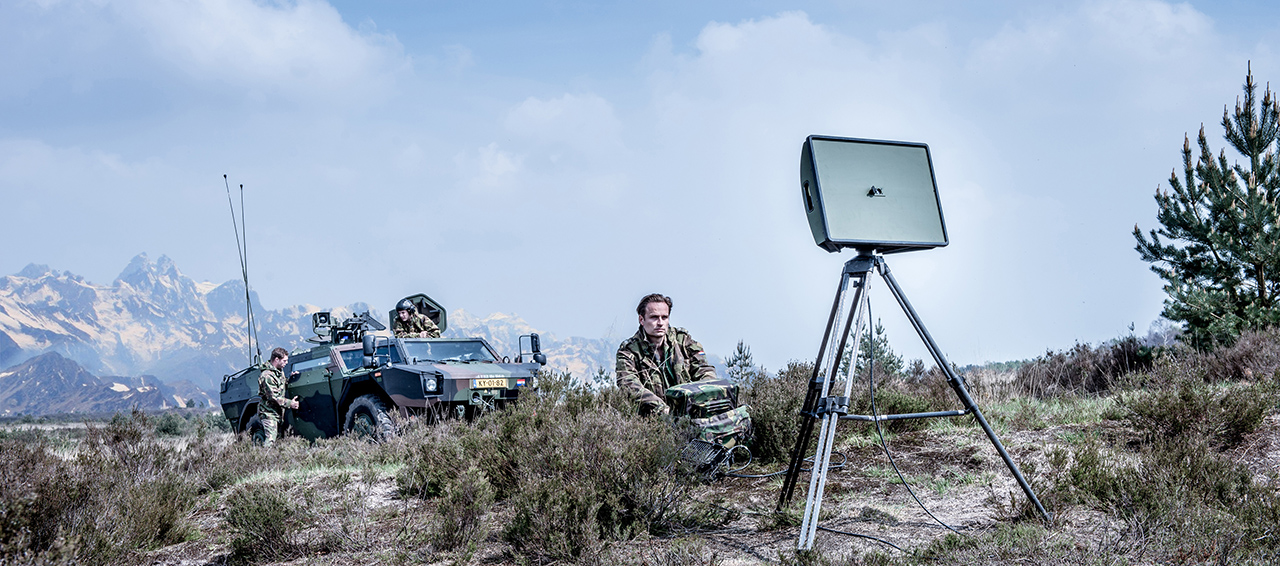
\includegraphics[width=\textwidth]{radar}
\captionof{figure}{Le radar portable Squire de Thales Air Systems}

Il existe néanmoins certains drones construits en carbone pouvant être perméables à certaines ondes radars et ainsi indétectable par cette technologie. Cependant le "radar passif", radar exploitant les variations d'ondes électromagnétiques en milieu urbain, telles que les ondes de la TNT, pourrait être exploité en milieu urbain.

\section{Synthèse}

Ainsi, la meilleure solution serait de réaliser un détecteur à base de ces trois modes de détection. C'est d'ailleurs pourquoi les produits les plus performants existant sur le marché utilisent un mélange de ces trois technologies. On peut notamment citer le cas du système drone-detector \cite{dronedetector}.

Néanmoins nous avons choisi pour ce projet de nous concentrer, dans un premier temps, sur une détection uniquement à base de radiogoniométrie.

% Ici il va falloir préciser plusieurs choses sur pourquoi ce choix. Notamment en précisant qu'on suppose que les drones respectent la réglementation, etc... 



%%% Local Variables: 
%%% mode: latex
%%% TeX-master: "rapport_analyse"
%%% End: 
